\chapter{Introducción específica} % Main chapter title

\label{Chapter2}

%----------------------------------------------------------------------------------------
%	SECTION 1
%----------------------------------------------------------------------------------------
En este capítulo se presentan las herramientas usadas para desarrollar el trabajo y un breve compendio de otros trabajos similares en la temática. Hacia el final, se encuentran los requerimientos y la planificación utilizada.

\section{Entorno de desarrollo}
\subsection{Hololens2}

El equipo que se utilizo para la interfaz de realidad aumentada es el Microsoft Hololens 2. Podemos ver una foto del equipo en la figura \ref{fig:hololens2}:

\begin{figure}[htpb]
	\centering
	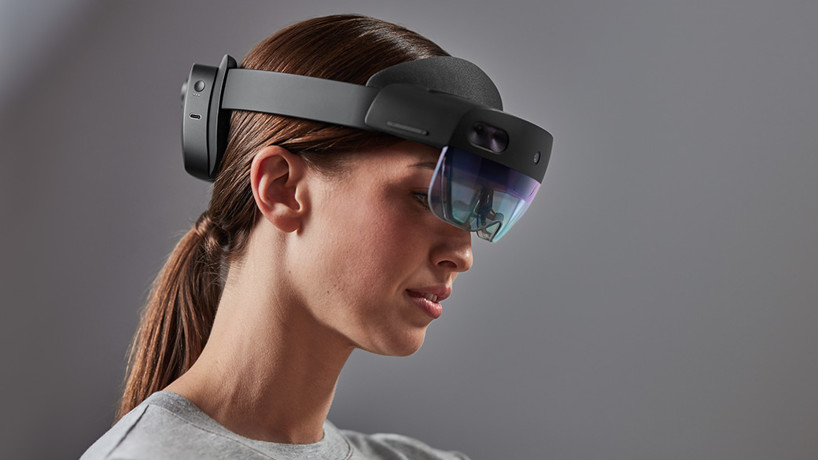
\includegraphics[scale=.5]{./Figures/hololens2.jpeg}
	\caption{hololens2\protect\footnotemark.}
	\label{fig:hololens2}
\end{figure}

\footnotetext{Imagen tomada de \url{https://img-prod-cms-rt-microsoft-com.akamaized.net/cms/api/am/imageFileData/}}


Fue lanzado al mercado para uso corporativo, Microsoft apuesta a que la tecnología sea usada con fines productivos en distintas industrias. Es un equipo de ultima generación que funciona con un sistema operativo Windows 10 core.  La tabla \ref{tab:holotab}, muestra sus especificaciones técnicas:

\begin{table}[htpb]
	\centering
	\caption[Hardware Hololens 2]{Especificaciones técnicas}
	\scalebox{0.9}{
	\begin{tabular}{l c c}    
		\toprule
		\textbf{Hardware} 	 & \textbf{Descripción}  \\
		\midrule
		Procesador				&  Qualcomm Snapdragon 850 \\		
		Memoria	 				&  4 GB DRAM \\
		Almacenamiento	 		&   64 GB \\
		Cámara	 				&   1080p \\
		Peso 	 				&   566 gr \\
		CPU holografica			&   Segunda generación\\
		Resolución				&   2k 3:2\\
		Unidad de medida inercial			&   Acelerómetro, giroscopio y magnetómetro\\
		Seguimiento de cabeza	&   4 cámaras de luz visible\\
		Seguimiento de ojos	&   2 cámaras de infrarrojas\\
		\bottomrule
		\hline
	\end{tabular}}
	\label{tab:holotab}
\end{table}

Lo innovador de su diseño es que utiliza micro espejos para proyectar 3 haces de luz láser de color rojo, verde y azul. Con un micro espejo por cada ojo oscilando a 12.000 veces por segundo, compone la imagen horizontal. Con un segundo micro espejo, oscilando a 120 veces por segundo forma la componente vertical. Luego,este haz de luz es proyectado hacia nuestra retina, utilizando el visor del Hololens 2 que actúa como una guía de onda. En la figura \ref{fig:Lasers} podemos ver una ejemplificación del funcionamiento interno:

\begin{figure}[htpb]
	\centering
	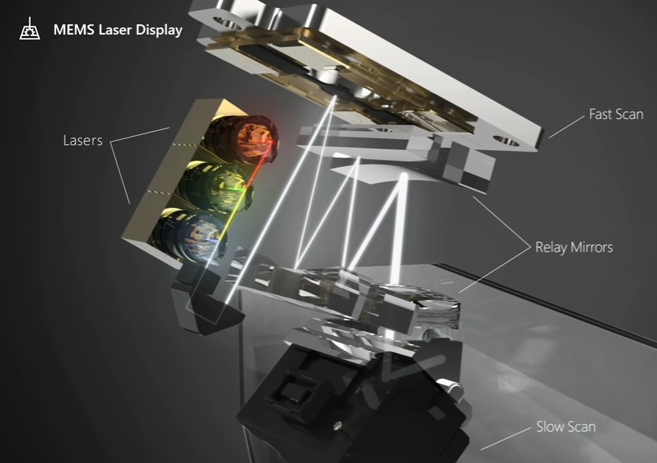
\includegraphics[width=\textwidth]{./Figures/Lasers.png}
	\caption{micro espejos\protect\footnotemark.}
	\label{fig:Lasers}
\end{figure}

\footnotetext{Imagen tomada de \url{https://img-prod-cms-rt-microsoft-com.akamaized.net/cms/api/am/imageFileData/}}


\subsection{MRTK}

MRTK(\textit{Mixed Reality Toolkit}) para Unity es un kit de desarrollo multiplataforma de código abierto para aplicaciones de realidad mixta. Proporciona un sistema de entrada multiplataforma, componentes fundamentales y bloques de construcción comunes para interacciones espaciales. Tiene como objetivo acelerar el desarrollo de aplicaciones para Microsoft HoloLens, los visores inmersivos de Windows Mixed Reality y la plataforma OpenVR. El proyecto busca reducir las barreras de entrada, crear aplicaciones de realidad mixta y contribuir a la comunidad. El \textit{framework} puede desglosarse conceptualmente como se muestra en la \ref{fig:mrtk}:

\begin{figure}[htpb]
	\centering
	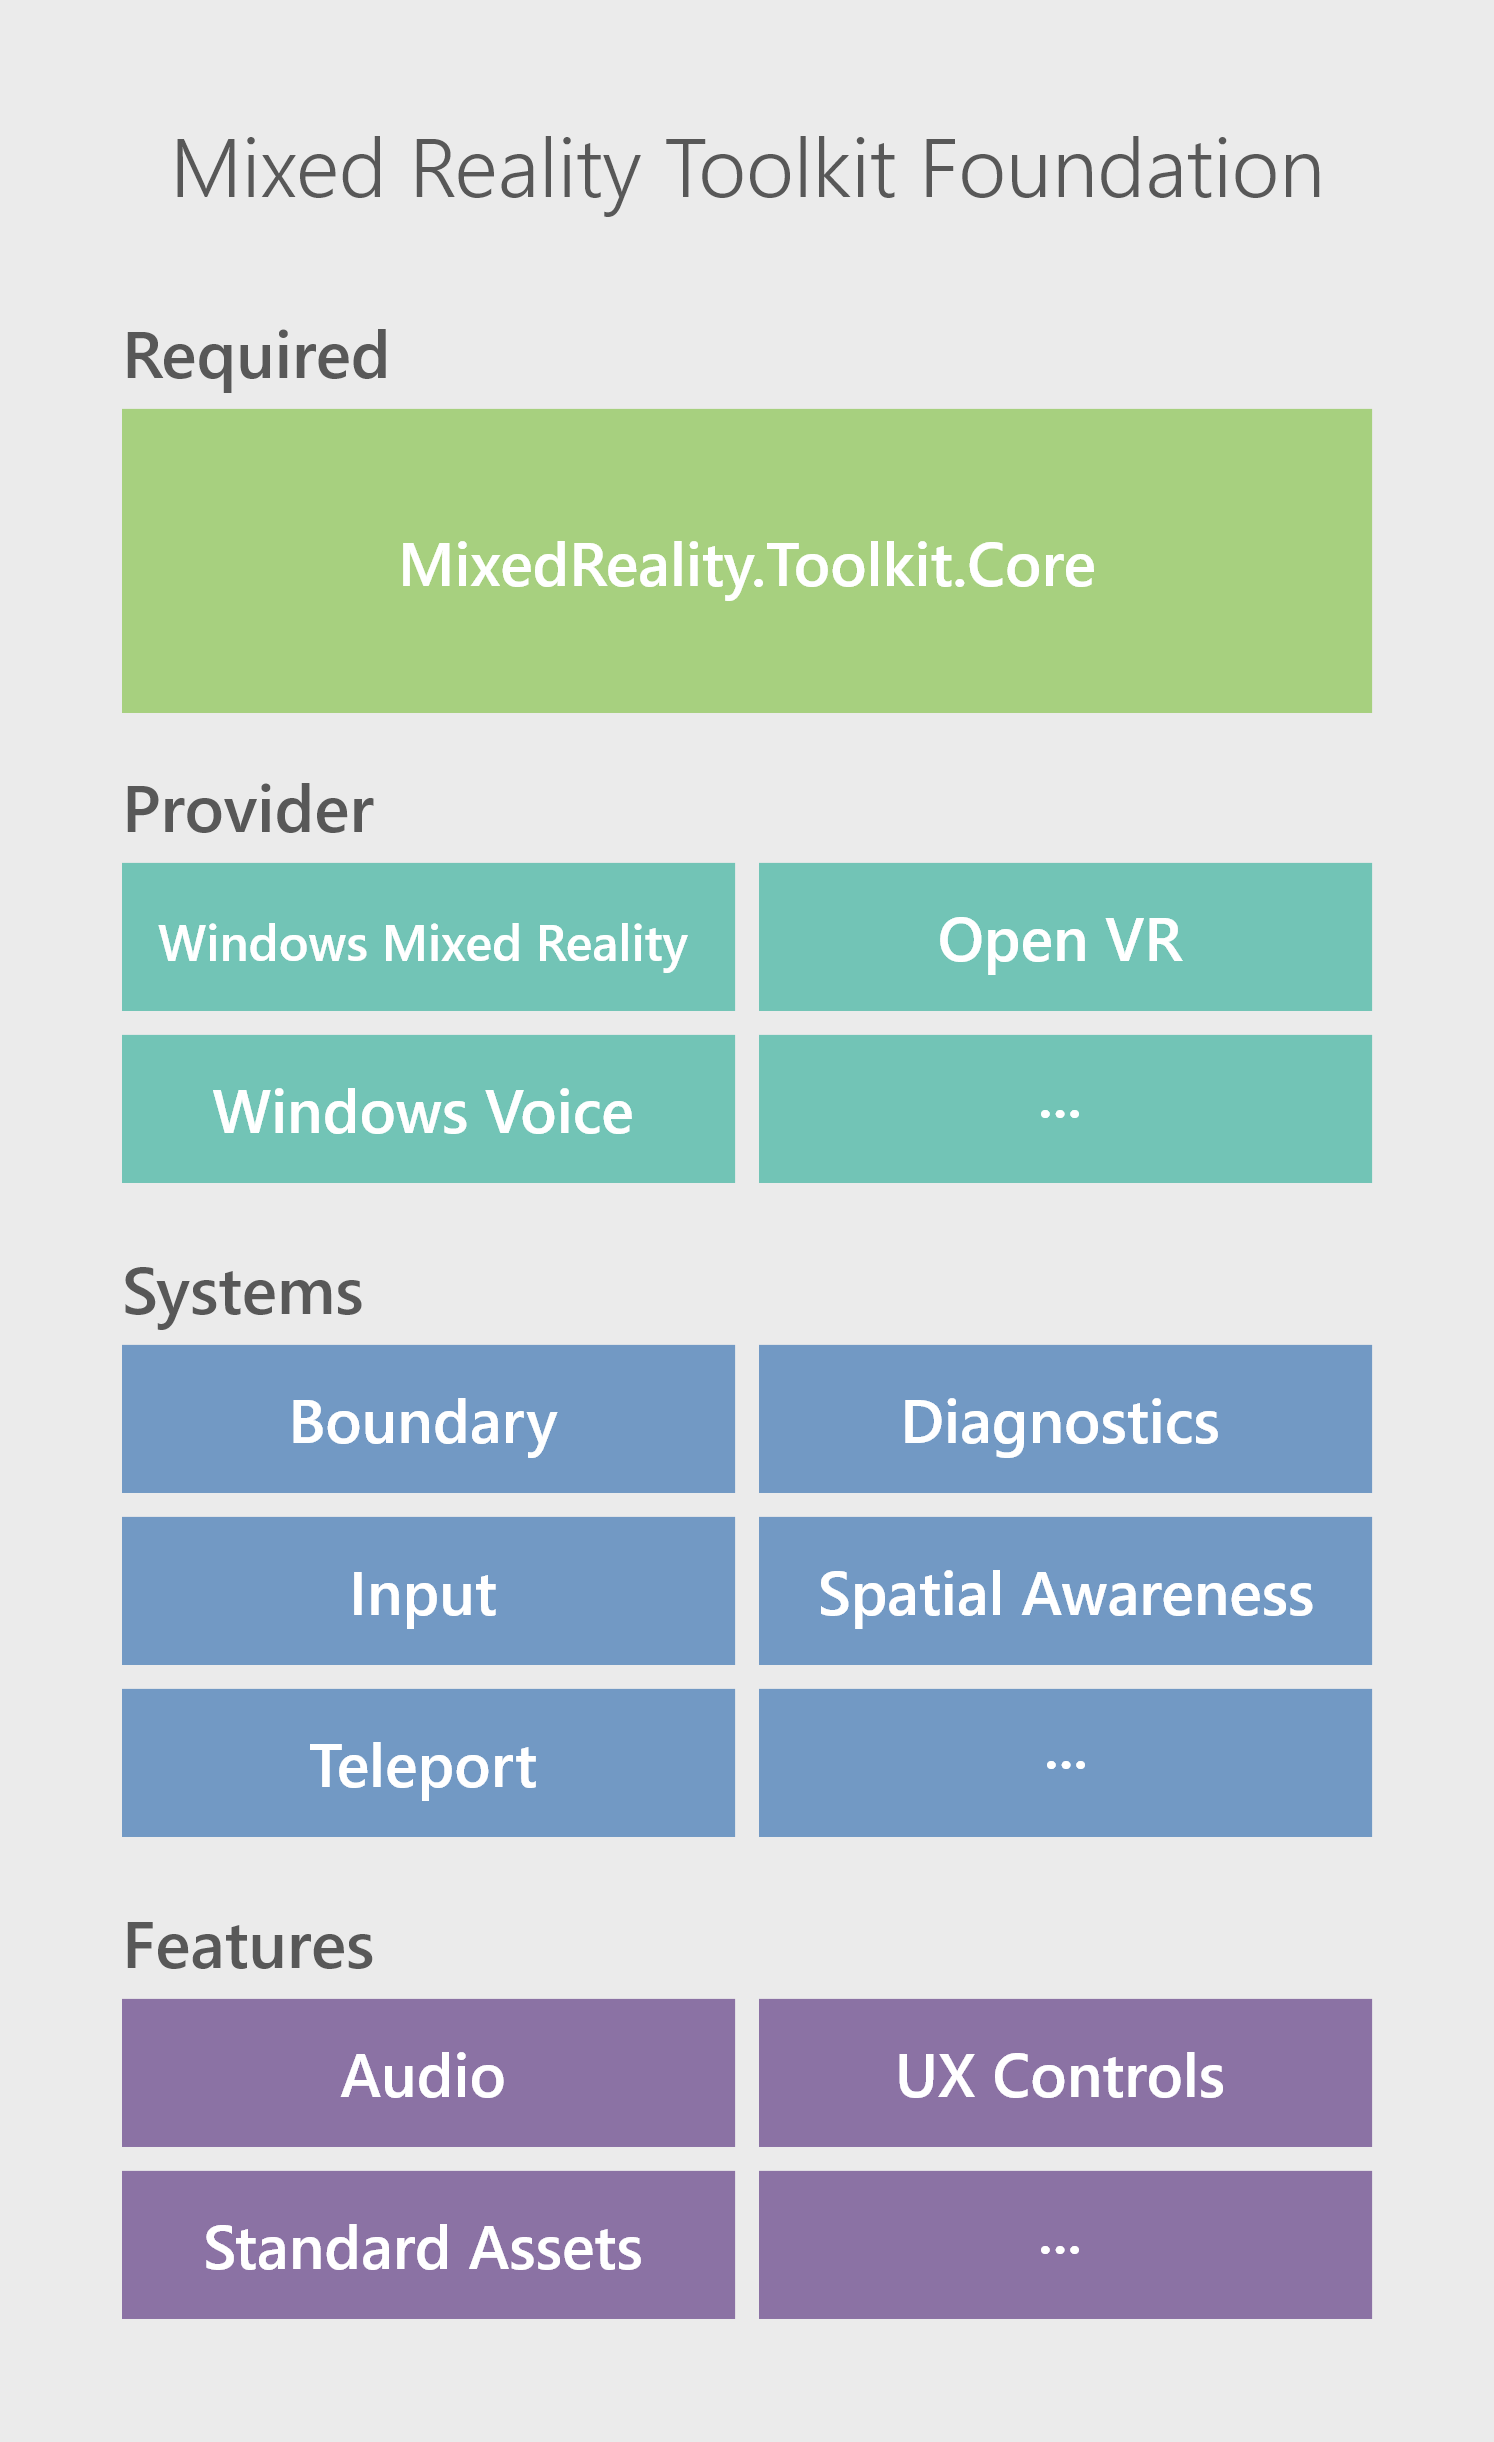
\includegraphics[scale=0.1]{./Figures/mrtk.png}
	\caption{componentes del \textit{framework} \protect\footnotemark.}
	\label{fig:mrtk}
\end{figure}

\footnotetext{Imagen tomada de \url{https://docs.microsoft.com/en-us/windows/mixed-reality/}}

Sus componentes principales son:
\begin{itemize}
\item \textit{Hands}: clase básica de soporte con servicios para seguimiento de las manos.
\item \textit{ObjectMeshObserver}: procesamiento del ambiente usando el modelado 3D.
\item \textit{WindowsMixedReality}:compatibilidad con dispositivos \textit{Windows Mixed Reality}, incluidos Microsoft HoloLens y auriculares inmersivos.
\item \textit{Profiles}: perfiles predeterminados para los sistemas y servicios de \textit{Microsoft Mixed Reality Toolkit}.
\item \textit{SceneSystem}: sistema que proporciona compatibilidad con aplicaciones de múltiples escenas..
\item \textit{StandardAssets}: renderizado estándar, materiales básicos y otros activos para experiencias de realidad mixta
\end{itemize}

Ademas del MRTK, se utilizan programas de diseño como el Fusion360 para crear objetos 3D. Se utiliza el Visual Studio como IDE de desarrollo y como herramienta de compilación. Y finalmente Unity, como herramienta de diseño visual de la aplicación. En la figura \ref{fig:workflow}, podemos ver un diagrama del entorno completo:

\begin{figure}[htpb]
	\centering
	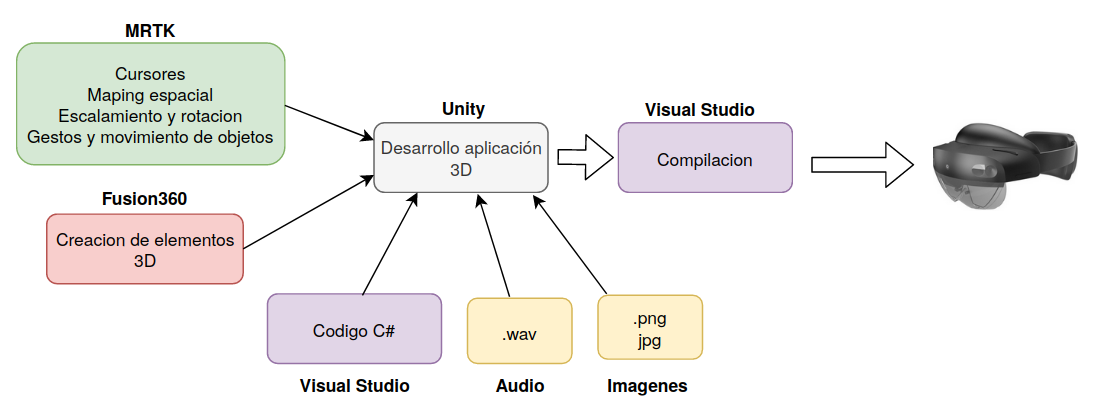
\includegraphics[width=\textwidth]{./Figures/workflow.png}
	\caption{entorno de desarrollo\protect\footnotemark.}
	\label{fig:workflow}
\end{figure}

\footnotetext{Imagen tomada de \url{https://img-prod-cms-rt-microsoft-com.akamaized.net/cms/api/am/imageFileData/}}

\subsection{OPC \textit{framework}}

Las especificaciones de OPC \textit{Classic} se basan en la tecnología de Microsoft Windows, utilizando COM / DCOM (\textit{Distributed Component Object Model}) para la comunicación entre componentes de software en una red distribuida cliente-servidor. La especificación original es OPC-DA (\textit{Data Access}), que define una interfaz entre las aplicaciones cliente y servidor para intercambiar datos de proceso y fabricación. Antes de OPC-DA, los productos de distintos proveedores (PLC, HMI) requerían que cualquier dispositivo o aplicación que se conectara a ellos, tuviera un ``controlador personalizado'' que comunicara el dispositivo con equipos de terceros. En la figura \ref{fig:OPCAQ} se muestra una arquitectura típica de control previa a la existencia del \textit{standard} OPC:

\begin{figure}[htpb]
	\centering
	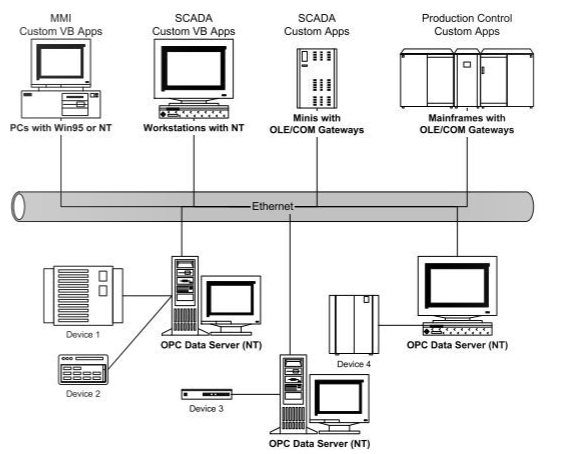
\includegraphics[scale=0.40]{./Figures/opc_1.png}
	\caption{arquitectura OPC\protect\footnotemark.}
	\label{fig:OPCAQ}
\end{figure}

\footnotetext{Imagen tomada de \url{https://technosoftware.com/opc-daaehda-client-net}}

Hubo muchos problemas asociados con las comunicaciones basadas en controladores personalizados. La tecnología patentada de alto costo que forzaba a los usuarios a mantener un proveedor en particular. Dificultades para configurar y  mantener actualizado los \textit{drivers} debido al lanzamiento de nuevos dispositivos y aplicaciones. OPC-DA hizo posible la conexión a cualquier fuente de datos en tiempo real sin un driver escrito específicamente para el par fuente de datos / receptor de datos. Por lo tanto, las lecturas y escrituras se pueden realizar sin que el receptor de datos tenga que conocer el protocolo nativo de la fuente de datos o la estructura de datos interna.\\ 

La especificación describe los objetos y sus interfaces, las cuales son implementadas por los servidores OPC. Aunque OPC está diseñado principalmente para acceder a datos desde un servidor en red, las interfaces se pueden utilizar en muchos lugares dentro de una aplicación. En el nivel más bajo, pueden obtener datos sin procesar de los dispositivos físicos y enviarlos a un SCADA o DCS, o desde el sistema SCADA o DCS a la aplicación. La arquitectura y el diseño permiten que una aplicación cliente acceda a datos de muchos servidores OPC proporcionados por distintos proveedores. En la figura \ref{fig:OPCbloques} se muestra un diagrama en bloques para ejemplificar lo explicado:

\begin{figure}[htpb]
	\centering
	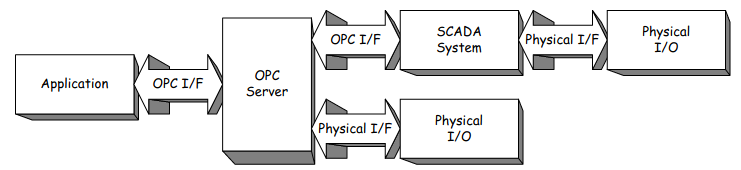
\includegraphics[scale=0.4]{./Figures/opc_2.png}
	\caption{diagrama en bloques\protect\footnotemark.}
	\label{fig:OPCbloques}
\end{figure}

\footnotetext{Imagen tomada de \url{https://opcfoundation.org}}

A alto nivel, un servidor OPC se compone de varios objetos: el servidor, el grupo y el elemento. El objeto del servidor OPC mantiene información sobre el servidor y sirve como contenedor para los objetos del grupo. El objeto del grupo mantiene información sobre sí mismo y proporciona el mecanismo para contener y organizar lógicamente los elementos OPC. Un cliente se comunica con el servidor a través de las interfaces para cada objeto OPC, como se ve en la figura \ref{fig:OPCapi}:

\begin{figure}[htpb]
	\centering
	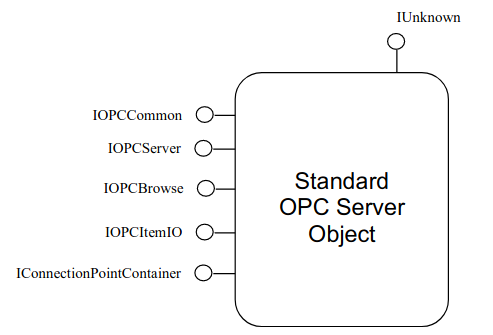
\includegraphics[scale=0.4]{./Figures/opc_3.png}
	\caption{diagrama en bloques\protect\footnotemark.}
	\label{fig:OPCapi}
\end{figure}

\footnotetext{Imagen tomada de \url{https://opcfoundation.org}}

\begin{itemize}
\item IOPCServer:ésta es la interfaz principal de un servidor OPC, permite realizar las consultar a los grupos de elementos OPC.
\item IUnknown: consiste en un puntero a una tabla que permite descubrir dinámicamente si un objeto admite una interfaz en particular.
\item IOPCCommon:Proporciona la capacidad de configurar y consultar el LocaleID para la sesión cliente/servidor en particular. El LocaleID contempla el formato de números, fechas, moneda, etc. puede depender de la configuración regional.
\item IOPCBrowse: proporciona métodos mejorados para navegar por el espacio de direcciones del servidor y para
obtener propiedades de los elementos OPC.
\item IConnectionPointContainer: permite disparar eventos llamando a un método de la interfaz de un objeto COM del lado del cliente implementado por el mismo cliente.
\item IOPCItemIO: en términos de rendimiento esta interfaz se comportará como si se creara un grupo, se agregaran los elementos OPC, se realizara una sola lectura o escritura y luego se eliminara el grupo. Por lo tanto no es la interfaz recomendada para la mayoría de las aplicaciones.
\end{itemize}

Los grupos OPC proporcionan una forma para que los clientes organicen los datos. Por ejemplo, el grupo puede representar elementos en una pantalla de operación o variables de un lazo PID. Los datos se pueden leer y escribir. Los elementos OPC representan conexiones a fuentes de datos dentro del servidor. Un elemento OPC, desde la perspectiva de la interfaz, no es accesible como objeto por un cliente OPC. Por lo tanto, no hay una interfaz externa definida para un elemento OPC. Todo el acceso a los elementos OPC se realiza a través de un objeto de grupo que ``contiene'' los elementos. Un grupo también proporciona una forma para que el cliente se ``suscriba'' a la lista de elementos para que pueda ser notificado cuando cambien. Este ratio de actualización es un parámetro configurable del servidor.


\subsection{Requerimientos}

A continuación se listan los requerimientos en base a las distintas etapas del trabajo:

\begin{enumerate}
\item Requerimientos asociados al desarrollo de la interfaz visual:
	\begin{enumerate}
	\item La interfaz debe ser intuitiva y simple.
	\item El idioma definido es Español.
	\end{enumerate}
\item Requerimientos asociados al desarrollo de lógica en .NET:
	\begin{enumerate}
	\item La aplicación debe ser fluida y responder sin demoras apreciables por el operador, estableciéndose así el límite máximo de espera en 2 segundos.
	\item La aplicación debe poder hacer operaciones GET y POST sobre un servidor web, ya sea local o en la nube.
	\end{enumerate}
\item Requerimientos asociados a la API rest:
	\begin{enumerate}
	\item La API no será de acceso público, solo podrá ser consultada por las aplicaciones que poseen un \textit{token} de seguridad.
	\end{enumerate}
\item Requerimientos asociados a la interfaz de comunicación con el sistema de control:	
	\begin{enumerate}	
	\item La solución debe poder consultar una serie de datos específicos a elección, de los elementos que pertenecen al sistema de control.
	\item La comunicación debe cumplir con el \textit{standard} OPC.
	\end{enumerate}
\end{enumerate}

\subsection{Planificación}

El trabajo fue dividido en tareas y se estimaron los tiempos que debían emplearse para cada una de ellas. A su vez, se analizaron qué tareas debían realizarse primero y cuáles eran sus dependencias. Al momento de organizar las tareas se consideraron 15 horas semanales efectivas de trabajo, obteniendo como resultado la planificación de la figura \ref{figure:gantt}:

\begin{figure}[htpb]
	\centering
	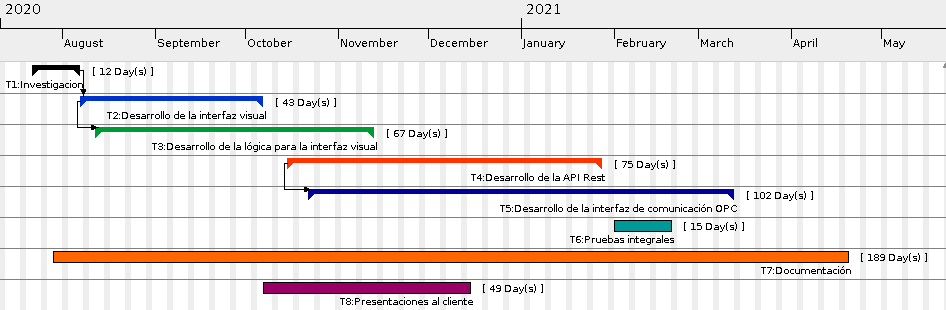
\includegraphics[width=14cm]{./Figures/gantt_1.png}
	\caption{diagrama de Gantt\protect\footnotemark.}
	\label{figure:gantt}
\end{figure}

Como se estimo al inicio del trabajo la comunicación OPC fue la que mas tiempo empleo, incluso se extendió 1 mes mas de lo planeado. 